\documentclass[border=6pt]{standalone}
% Shared preamble for web figures.  Each figure is a standalone .tex that
% \input's this file; scripts/make-figures.sh turns it into an SVG.
% Handouts pull the same file with \fig{Unit_X/<name>}.
\usepackage[T1]{fontenc}
\usepackage{helvet}
\renewcommand{\familydefault}{\sfdefault}
\renewcommand{\ttdefault}{pcr}  % Courier: a real Type 1 typewriter font
\usepackage{amsmath}
\usepackage{tikz}
\usetikzlibrary{arrows.meta,positioning,calc,shapes.symbols,shapes.geometric}

% Who makes the rules is the point of most diagrams in this book, so the
% colors mean the same thing everywhere: blue is a person, orange is the
% computer, green is an answer, pink is the human brain.
\definecolor{person}{HTML}{2C6FAE}
\definecolor{machine}{HTML}{D35400}
\definecolor{result}{HTML}{1E8449}
\definecolor{brainpink}{HTML}{C2185B}
\definecolor{ink}{HTML}{2C3E50}

\tikzset{
  doodle/.style={line width=1.5pt, line cap=round, line join=round, draw=ink},
  box/.style={draw, rounded corners=5pt, line width=1.1pt, align=center,
              inner sep=7pt, minimum height=1.0cm, font=\small},
  personbox/.style={box, draw=person, fill=person!10},
  machinebox/.style={box, draw=machine, fill=machine!10},
  resultbox/.style={box, draw=result, fill=result!10},
  plainbox/.style={box, draw=ink!70, fill=ink!4},
  flow/.style={-{Stealth[length=8pt]}, line width=1.4pt, draw=ink},
}

% A person (blue) and a robot head (orange) as small icons.
% \personicon{x}{y}{scale}   \roboticon{x}{y}{scale}
\newcommand{\personicon}[3]{%
  \begin{scope}[shift={(#1,#2)}, scale=#3]
    \fill[person] (0,0.62) circle (0.28);
    \fill[person, rounded corners=6pt] (-0.42,-0.55) rectangle (0.42,0.28);
  \end{scope}}
\newcommand{\roboticon}[3]{%
  \begin{scope}[shift={(#1,#2)}, scale=#3]
    \draw[machine, line width=1.2pt] (0,0.5) -- (0,0.72);
    \fill[machine] (0,0.78) circle (0.08);
    \draw[machine, line width=1.4pt, fill=machine!12, rounded corners=4pt] (-0.5,-0.45) rectangle (0.5,0.5);
    \fill[ink] (-0.2,0.12) circle (0.08);
    \fill[ink] (0.2,0.12) circle (0.08);
    \draw[ink, line width=1pt] (-0.22,-0.22) -- (0.22,-0.22);
  \end{scope}}

\begin{document}
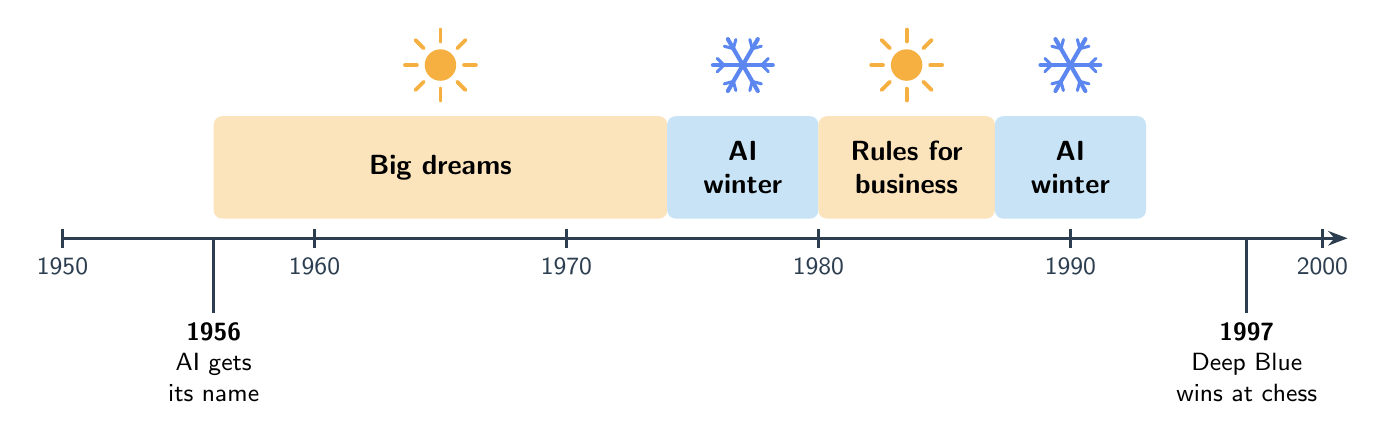
\begin{tikzpicture}[x=0.32cm, y=1cm]
% Big dreams and AI winters, 1950 to 2000.  Winter dates are the usual
% rough ones: 1974-1980 and 1987-1993.
\definecolor{sunny}{HTML}{F5B041}
\definecolor{icy}{HTML}{85C1E9}
\newcommand{\sun}[2]{\begin{scope}[shift={(#1,#2)}]
  \fill[sunny] (0,0) circle (0.2cm);
  \foreach \a in {0,45,...,315} \draw[sunny, line width=1.4pt, line cap=round] (\a:0.3cm) -- (\a:0.45cm);
\end{scope}}
\newcommand{\snow}[2]{\begin{scope}[shift={(#1,#2)}]
  \foreach \a in {0,60,...,300} {
    \draw[icy!70!blue, line width=1.5pt, line cap=round] (0,0) -- (\a:0.38cm);
    \draw[icy!70!blue, line width=1.1pt, line cap=round] (\a:0.24cm) -- ++({\a+45}:0.12cm) (\a:0.24cm) -- ++({\a-45}:0.12cm);
  }
\end{scope}}
% bands (x is the year minus 1950)
\fill[sunny!35, rounded corners=3pt] (6,0.25) rectangle (24,1.55);
\fill[icy!45, rounded corners=3pt] (24,0.25) rectangle (30,1.55);
\fill[sunny!35, rounded corners=3pt] (30,0.25) rectangle (37,1.55);
\fill[icy!45, rounded corners=3pt] (37,0.25) rectangle (43,1.55);
\sun{15}{2.2} \node[font=\bfseries] at (15,0.9) {Big dreams};
\snow{27}{2.2} \node[font=\bfseries, align=center] at (27,0.9) {AI\\winter};
\sun{33.5}{2.2} \node[font=\bfseries, align=center] at (33.5,0.9) {Rules for\\business};
\snow{40}{2.2} \node[font=\bfseries, align=center] at (40,0.9) {AI\\winter};
% axis
\draw[ink, line width=1.2pt, -{Stealth[length=7pt]}] (0,0) -- (51,0);
\foreach \y in {1950,1960,1970,1980,1990,2000} {
  \pgfmathtruncatemacro{\x}{\y-1950}
  \draw[ink, line width=1pt] (\x,0.12) -- (\x,-0.12) node[below, font=\small] {\y};
}
% events
\draw[ink, line width=1pt] (6,0) -- (6,-0.95);
\node[anchor=north, align=center, font=\small] at (6,-0.95) {\textbf{1956}\\AI gets\\its name};
\draw[ink, line width=1pt] (47,0) -- (47,-0.95);
\node[anchor=north, align=center, font=\small] at (47,-0.95) {\textbf{1997}\\Deep Blue\\wins at chess};
\end{tikzpicture}
\end{document}
